\section{Description of Task 1, DC-motor}

The second system that is described is the inverted pendulum.

\begin{figure}[h]
    \centering
    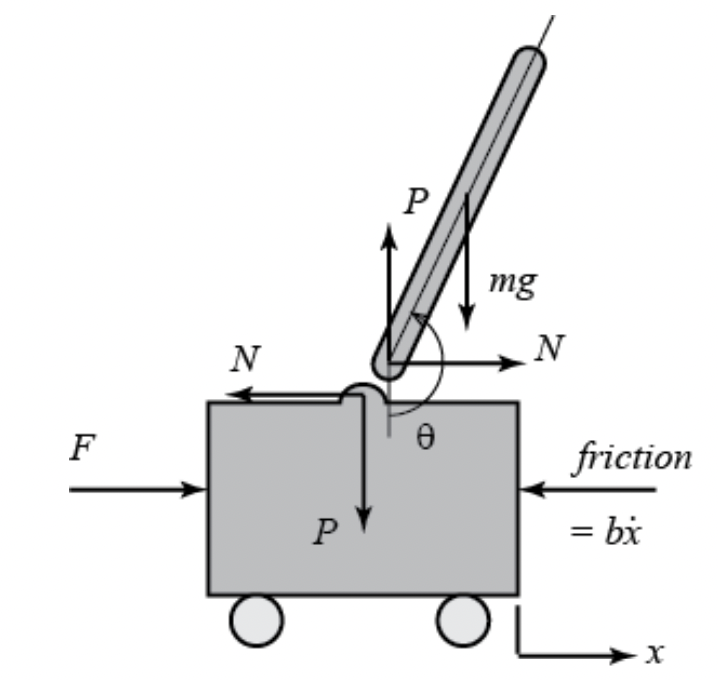
\includegraphics[width = 0.5\textwidth]{Images/InvPendulum.png}
    \caption{Schematic of the inverted pendulum system}
    \label{fig:InvPendulum}
\end{figure}

The systems transcerfunction is given by:
\begin{equation}
    P_{pend}(s) = \frac{\Phi (s)}{U(s)} = \frac{\frac{ml}{q} s}{s^3 + \frac{b(I+ml^2)}{q}s^2 - \frac{(M+m)mgl}{q} s - \frac{bmgl}{q} }
\end{equation}
\begin{equation}
    q = (M+m)(I+ml^2)-(ml)^2
\end{equation}

\begin{center}
\begin{tabular}{ |c|c|c|c|}

\hline
Parametre & Symbol & Value & Unit \\
\hline
Cart mass & M & 9 & Kg\\ 
\hline
Pendulum mass & m & 1 & Kg \\  
\hline
Length to pendulum CoM & l & 1 & m \\
\hline
Pendulum moment of inertia & I & 9.1 & $Kgm^2$ \\
\hline
Gravity const & g & 10 & m/$s^2$ \\
\hline
Cart friction coefficient & b & 100 & N/ms \\
\hline
\end{tabular}
\label{tab:Parameters}
\end{center}